\section{NEON}
To improve the performance of media and signal processing, 
\emph{NEON} SIMD technology is implemented in \emph{Cortex-A8} core of \emph{OMAP 3530} GPP. 
\emph{NEON} SIMD technology, which is also known as Advanced SIMD extension, 
takes the advantage of parallel operation to achieve the speed up.
\subsection{SIMD}
To understand NEON technology, the idea of SIMD is introduced at first. 
SIMD (Single Instruction Multiple Data) describes a way to perform the same operation on multiple data with same type and size in a single instruction. 
The idea of parallel operation comes from the fact that most of multimedia data are 16-bit or 8-bit wide, while the general purpose registers are 32-bit wide. 
To effectively utilize the space of registers, simultaneous computation is developed.  
\subsection{NEON Technology} 
\emph{NEON} technology, as the Advanced SIMD extension in \emph{Cortex-A8}, performs SIMD operations in group. 
NEON instructions operate on vectors stored in 64-bit or 128-bit registers, 
then vectors of elements with same type can perform the same operation on multiple items at the same time.
Figure~\ref{fig:neon} shows how multiple items are computed simultaneously. 

\begin{figure}[h]
\centering
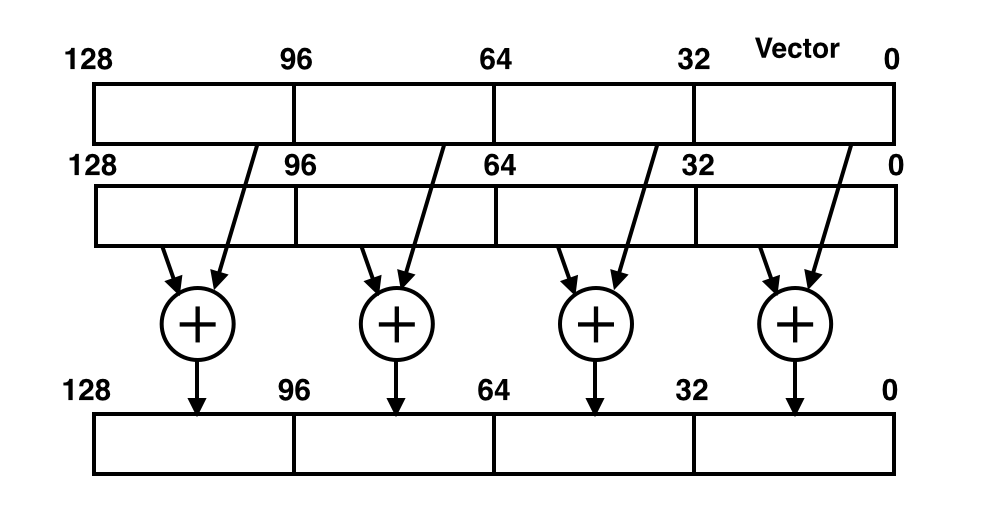
\includegraphics[width=0.9\textwidth]{images/neon}
\caption{Parallel computing based on NEON}
\label{fig:neon}
\end{figure}

\subsection{Hardware Features}
NEON architecture has the following features\cite{hardware}:
\begin{enumerate}
\item \emph{16-Entry instruction queue}
\item \emph{32 x 64-bit general purpose registers in register file}
These registers can alternatively be viewed as 16 x 128-bit registers
\item \emph{6-stage execution pipeline}
NEON supports either integer of single precision floating point execute pipeline.
\item \emph{Load/store and permute pipeline}
\item \emph{12–Entry load data queue}
\end{enumerate}

\subsection{Implementation}
To enable the build-in intrinsics of NEON, 
\emph{$-$mfpu$=$neon}\cite{ARMoptions} is used during compiling time.
Also, header file \emph{arm\_neon.h} is included 
to support NEON intrinsics in the c file.
In our case, the incoming message contains the matrix with data of 16-bit wide, 
and then after calculation, when the final outcome is sending back to GPP, data size is 32-bit to avoid overflow.
In the following, NEON intrinsics that are used for parallel computing in our experiment are explained.
\subsubsection{Vector Data Type}
Neon defined its own data type\cite{DataType} for multiple data operation, the format is given as:
~\\ 
\textbf{ \textless type\textgreater \textless size \textgreater x\textless number of lanes\textgreater\_t}

For example, the data type we are going to use in NEON is \emph{uint32x4\_t}, 
which means the vector has four lanes, 
with each of the them containing an unsigned 32-bit integer. 
\subsubsection{NEON Intrinsics}
NEON intrisics \cite{Intrinsics}provide groups of functions for operation. 
In our case, functions related to load, multiplication and addition are used. 
\begin{enumerate}
\item \textbf{uint32x4\_t  vmovq\_n\_u32(uint32\_t value)}

This intrinsic loads all lanes of vector to the same input value. 
The input value is an unsigned 32-bit integer, 
while the four lanes being loaded each contains an unsigned 32-bit as well.


\item \textbf{int32x4\_t   vld1q\_s32(\_\_transfersize(4) int32\_t const * ptr)}

This intrinsic loads a single value from memory to all lanes.
The data stored in memory is signed 32-bit integer, 
while the four lanes each contains a signed 32-bit integer.

\item \textbf{int32x4\_t   vmlaq\_s32(int32x4\_t a, int32x4\_t b, int32x4\_t c)}

This intrinsic multiplies b by c, and accumulates the result with a in all four lanes.
The final results are then stored in four lanes as well.
\end{enumerate}

\subsubsection{Multiplication Algorithm}

In order to fully utilize the Neon resources, we have used following algorithm to compute the matrix multiplication. The following illustration shows one rows of results.
The input matrices are following:

$$
\begin{pmatrix}
 x1 	& \color{red}{x2} 	& \color{green}{x3} & \color{blue}{x4}\\
 x5 	& x6 				& x7&x8\\
 x9 	& x10 				& x11&x12\\
 x13 	& x14 				& x15&x16\\
\end{pmatrix}
\times
\begin{pmatrix}
y1&y2&y3&y4\\
y5&y6&y7&y8\\
y9&y10&y11&y12\\
y13&y14&y15&y16\\
\end{pmatrix}
$$


The output matrix would be : 
=
\begin{table}[h]
	\resizebox{\textwidth}{!}{
		$\left(
			\begin{tabular}{cccc}
				x1y1+\color{red}{x2}y5\color{black}{+}\color{green}{x3}y9\color{black}{+}\color{blue}{x4}y13&x1y2\color{black}{+}\color{red}{x2}y6\color{black}{+}\color{green}{x3}y10\color{black}{+}\color{blue}{x4}y14&x1y3\color{black}{+}\color{red}{x2}y7\color{black}{+}\color{green}{x3}y11\color{black}{+}\color{blue}{x4}y15&x1y4\color{black}{+}\color{red}{x2}y8\color{black}{+}\color{green}{x3}y12\color{black}{+}\color{blue}{x4}y16\\
				-&-&-&-\\-&-&-&-\\-&-&-&-\\
			\end{tabular}
		\right)$
	}
\end{table}

In the output matrix ,  the  elements with the same color are multiplied by the Neon at the same time. In this way, Neon produces the results of 4 multiplications at the same time.  In the above output row, x1y1, x1y2, x1y3 and x1y4 are produces by the neon simultaneously.  But these are just the partial results for the first row of output matrix. In order to get the complete results for the first row these partial results should be added to the other partial results  of the same row.  This complete task of multiplication and addition is done by using "Multiplication and Addition" functional unit of neon. The conceptual diagram of this multiplication and addition is shown in figure~\ref{fig:neon_mult_add}.
\begin{figure}[h]
\centering 
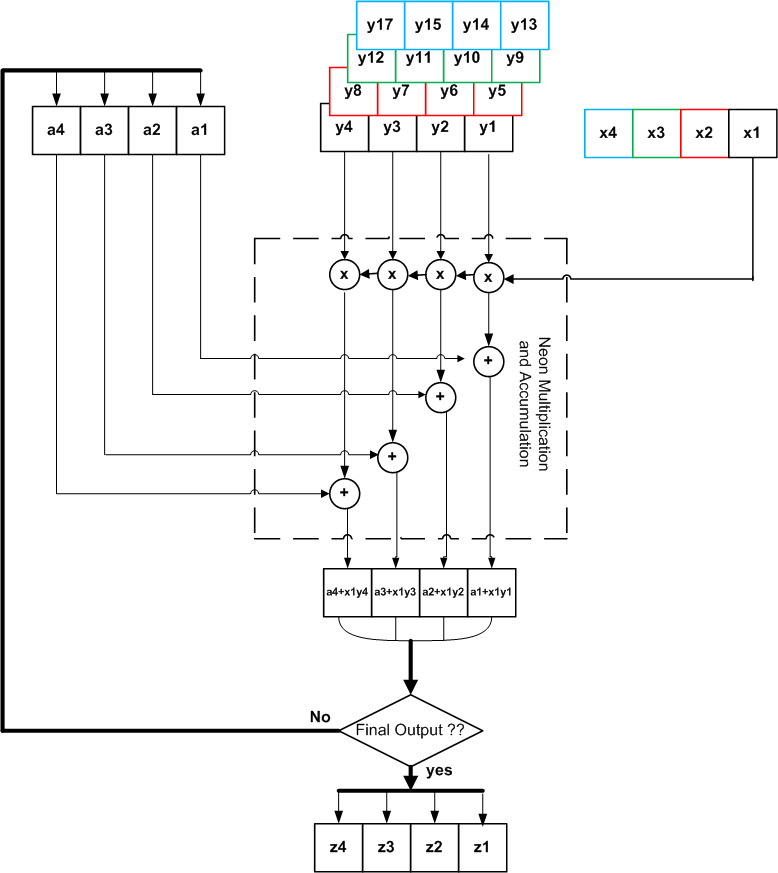
\includegraphics[width= 0.7\textwidth]{images/MandA}
\caption{Parallel Multiplication and Addition with Neon  }
\label{fig:neon_mult_add}
\end{figure}
